%!TEX root=thesis.tex

\chapter{Introduction}
\label{cha:intro}

\begin{figure}
  \centering
  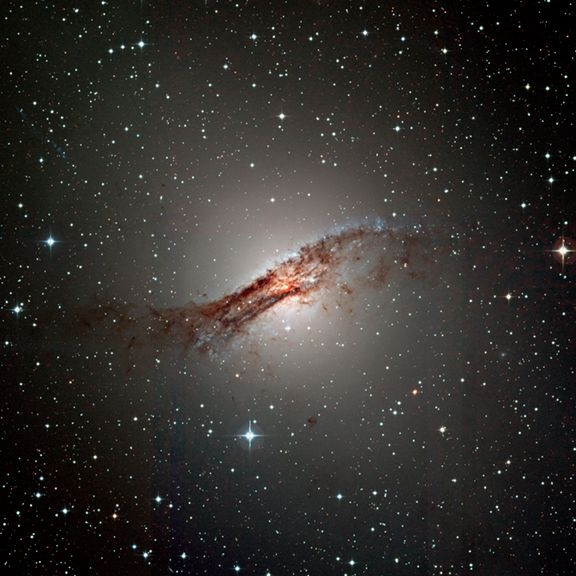
\includegraphics[width=0.24\textwidth]{images/centaurus_a_optical}
  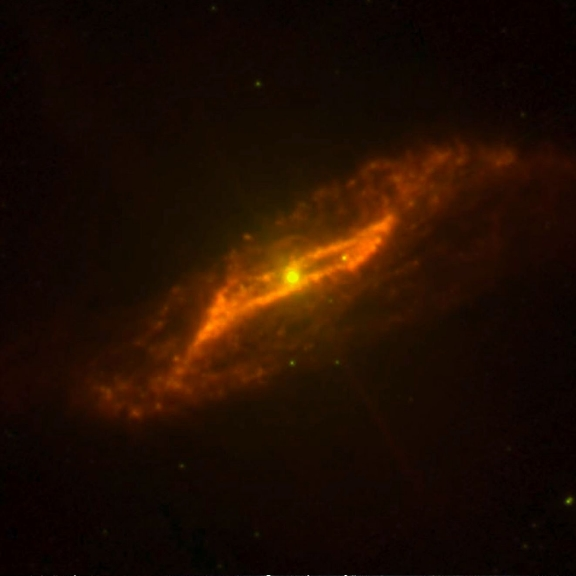
\includegraphics[width=0.24\textwidth]{images/centaurus_a_infrared}
  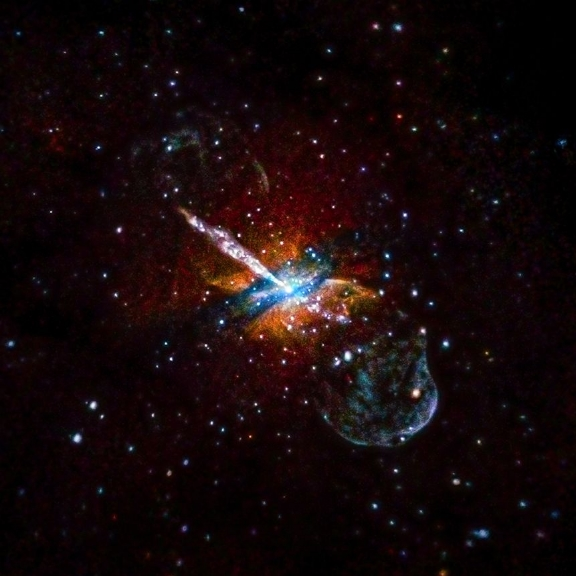
\includegraphics[width=0.24\textwidth]{images/centaurus_a_xray}
  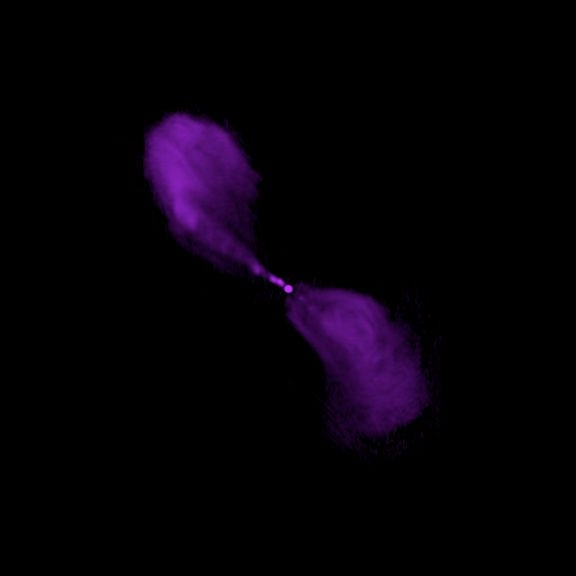
\includegraphics[width=0.24\textwidth]{images/centaurus_a_radio}
  \caption{Centaurus A in different wavelengths. From left to right: optical,
    infrared, X-ray, and radio. \emph{Image: ESO/WFI/M.Rejkuba et al. (Optical);
    NASA (Infrared); NASA/CXC/U.Birmingham/M.Burke et al. (X-ray);
    NSF/VLA/Univ.Hertfordshire/M.Hardcastle (Radio)}}
  \label{fig:different-wavelengths}
\end{figure}

Radio images of distant supermassive black holes offer unique insight into the
inner workings of galaxies and their environment. Newer, larger, and better
radio surveys will allow astronomers to learn more than ever before about these
objects. The galaxies in which black holes are found do not appear in radio
surveys (instead appearing in infrared surveys), but to fully investigate them,
astronomers need information about both the black hole and its host galaxy. This
leads to a difficult problem: How do we match our radio observations of
supermassive black holes to infrared observations of their host galaxies?

An object emits light at different wavelengths depending on its physical
properties. As such, looking at the sky in different wavelengths gives us very
different pictures. For example, Figure \ref{fig:different-wavelengths} shows
Centaurus A imaged in optical, infrared, X-ray, and radio light. The disc of
the galaxy is only visible in optical and infrared, and the large jets emitted
from the centre of the galaxy are only visible in X-ray and radio. This shows
that to fully understand an astronomical object, we have to look at it in many
different wavelengths.

While it is possible to look at one object in many wavelengths at once, we can
only do so for one object at a time. However, most astronomical data comes from
\emph{surveys}, where a telescope images large areas of the sky at once in
specific wavelengths. These surveys detect many objects, and individually
observing all of them is impractical. This leads us to the problem of
\emph{cross-identification}: Given an object detected at one wavelength, what
is the corresponding object at another wavelength?

\begin{figure}
  \centering
  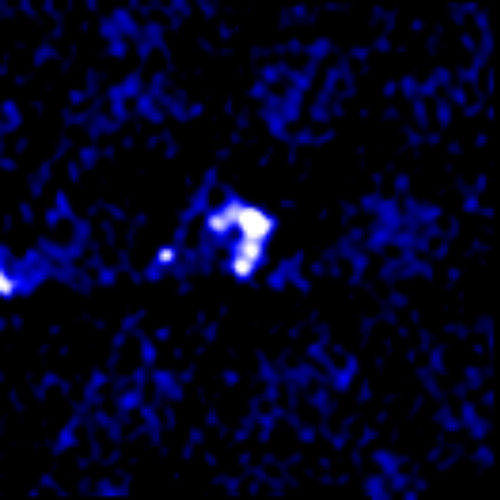
\includegraphics[width=0.3\textwidth]{images/first_FIRSTJ081509.0+270337.jpg}
  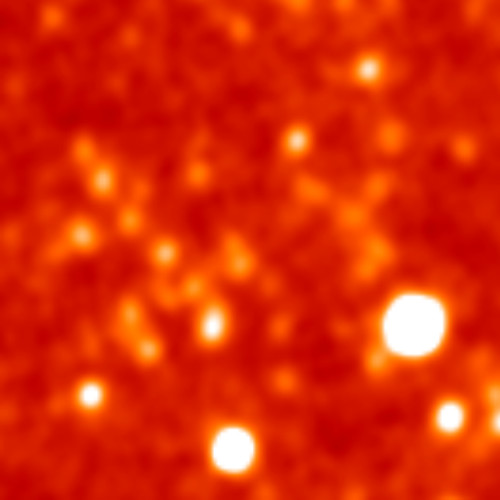
\includegraphics[width=0.3\textwidth]{images/wise_FIRSTJ081509.0+270337.jpg}
  \caption{The same patch of sky (8h 15m 9.0s +27$^\circ$ 3$'$ 37$''$) imaged in
    radio (left) and infrared (right). \emph{Image: NRAO VLA (Radio); WISE
    (Infrared)}}
  \label{fig:radio-ir-comparison}
\end{figure}

At first, this might sound easy. We could simply take note of the position of
the object in an image at one wavelength, and then match it to the same
position in an image at the other wavelength. This, however, assumes that
objects appear at the same position in multiple wavelengths. While this is
true for point-like objects, it is not true in general. Objects that are not
point-like may stretch across the sky, and only parts of the object may emit
each wavelength. We can again look to Centaurus A (Figure
\ref{fig:different-wavelengths}) as an example: The brightest part of
Centaurus A in infrared is far removed from the brightest parts in radio. When
objects are very distant, cross-identification becomes even harder. Figure
\ref{fig:radio-ir-comparison} shows the same patch of sky in both radio and
infrared. The infrared image shows no obvious counterpart for the object visible
in the radio image.

% Problems involved with cross-identification are compounded by Much like how
% the human eye can only see red, blue, and green light, telescopes can only
% see a limited number of

The cross-identification problem is compounded by the sheer size of the
universe. The scale of modern astronomical surveys is enormous: Astronomers
have catalogued millions of radio objects \citep{banfield15} and hundreds of
millions of infrared objects \citep{cutri13}. This makes manual
cross-identification impossible. Automated cross-identification algorithms
exist \citep{proctor06, fan15}, but are expected to fail for upcoming radio
surveys \citep{banfield15}.

The Evolutionary Map of the Universe (EMU) \citep{norris11} is one such survey.
EMU will use the new Australian SKA Pathfinder (ASKAP) telescope to image 75\%
of the sky in radio wavelengths, and is expected to find over 70 million radio
galaxies --- over 30 times the number of radio galaxies we know about today
\citep{banfield15}! These objects will need to be cross-identified with their
infrared counterparts, but it is estimated that 10\% of these radio galaxies
will be too complicated for current automated cross-identification algorithms
\citep{banfield15, norris11}.

% New telescopes are continually being developed, with higher resolutions and
% higher sensitivity than ever before. It is a particularly exciting time in radio
% astronomy: The Square Kilometre Array (SKA) \citep{ska}, an upcoming radio
% telescope, is expected to be built by 2024. It will be larger and faster than
% any previous radio telescope, and detect radio objects far dimmer and more
% distant than those we have detected thus far. Accordingly, it will produce huge
% amounts of data: over 160 terabytes of data per second \citep{ska}. Due to the
% scale of the SKA, many pathfinder projects have been launched to provide
% testbeds for new technologies to be used in the SKA and for new ways to handle
% the data that the SKA will produce. The Australian SKA Pathfinder (ASKAP) is one
% such project. It is a recently constructed radio telescope in Western Australia,
% and it will soon be used to conduct a number of new astronomical studies,
% including the Evolutionary Map of the Universe (EMU) \citep{norris11}. EMU is a
% radio survey of incredible size, covering 75\% of the sky at very high
% resolution and sensitivity. It is expected to find 30 times more radio galaxies
% than we have ever known before, bringing the total to over 70 million. These
% radio galaxies will need to be cross-identified with their infrared
% counterparts, and it is estimated that 10\% of these radio galaxies will be too
% complicated for current automated cross-identification algorithms
% \citep{banfield15, norris11}.

% \begin{figure}
%   \centering
%   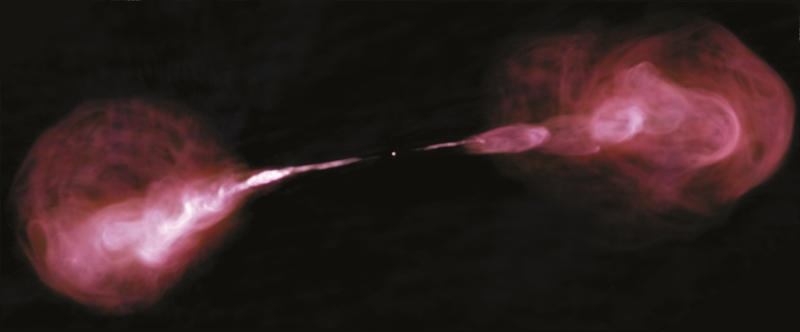
\includegraphics[width=0.8\textwidth]{images/herculesA.jpg}
%   \caption{Hercules A, a radio galaxy. We see jets emitted from the supermassive
%     black hole near the centre of the image. The galaxy itself is not visible in
%     radio wavelengths. \emph{Image: B. Saxton, W. Cotton and R. Perley
%     (NRAO/AUI/NSF)}}
%   \label{fig:radio-galaxy}
% \end{figure}

% Objects detected by EMU will need to be cross-identified with their counterparts
% in surveys at other wavelengths. Unfortunately, radio objects can be arbitrarily
% complex --- many radio objects are jets from supermassive black holes at the
% centre of galaxies, and these jets warp as they interact with their environment.
% An example of such an object is shown in Figure \ref{fig:radio-galaxy}. An
% estimated 10\% of EMU radio objects will be too complicated for current
% automated cross-identification algorithms \citep{banfield15, norris11}.

Radio Galaxy Zoo (RGZ) \citep{banfield15} is a citizen science project that
attempts to crowdsource the cross-identification problem. Volunteers are
presented with an image of the sky in both radio and infrared, and are asked to
identify radio objects and associate them with the corresponding infrared
object. The cross-identification interface is available online, so anyone can
help cross-identify radio objects\footnote{\url{https://radio.galaxyzoo.org/}}.

RGZ is based on the highly successful Galaxy Zoo \citep{lintott08, lintott11}.
The Zooniverse platform\footnote{\url{https://zooniverse.org/}} created by
Galaxy Zoo provides a way for non-experts to help researchers label data across
a wide range of scientific fields, and has resulted in well over 110
publications\footnote{See \url{https://www.zooniverse.org/about/publications}
for a full list.}.

To date, with the help of thousands of volunteers, RGZ has managed to
cross-identify over 100~000 radio galaxies. While this does not compare in scale
to EMU, the hope is that these cross-identifications can be used to train
next-generation machine learning algorithms.

\section{Contributions}
\label{sec:contributions}

  We present in this thesis a supervised learning approach to the problem of
  radio cross-identification, using label data sourced from the Radio Galaxy
  Zoo. Our approach is to frame the radio cross-identification problem as object
  localisation, and then as binary classification, allowing standard machine
  learning techniques to be applied to the problem. This is the first
  application of machine learning to automated radio cross-identification that
  we are aware of.

  Our methods do not make use of any astronomical models. We believe that this
  will help in the development of future algorithms for cross-identification of
  objects detected in EMU, where astronomical models may fail with the discovery
  of new classes of radio object. Instead of astronomical models, we use
  features extracted automatically from radio images using a convolutional
  neural network (Section \ref{sec:radio-features}). To our knowledge, this is
  the first instance where features have been automatically extracted from radio
  images.

  We have made use of the Radio Galaxy Zoo cross-identification database
  \citep{banfield15}. This is a very recent data set, and our work is one of the
  first uses of this data. In particular, this work is the first application of
  machine learning to labels from Radio Galaxy Zoo.

  In the process of developing our cross-identification methods, we have
  investigated the predictive power of infrared flux ratios, which are believed
  to correlate with whether a galaxy contains an AGN (Section
  \ref{sec:feature-analysis}) \citep{banfield15}. Further, we have shown that
  the features we have extracted from radio images are better predictors.

  We have implemented two prominent crowd learning algorithms by
  \citet{raykar10} and \citet{yan10}, and compared their performance against a
  simple crowd learning algorithm (logistic regression with majority vote,
  Sections \ref{sec:raykar} and \ref{sec:yan}). Our implementation is
  MIT-licensed, and is the only open-source implementation that we are aware of.

  In Chapter \ref{cha:active-learning} we have highlighted some problems with
  applying existing active learning and crowd learning literature to citizen
  science.

  Finally, we have implemented an open-source Python library for crowd-based
  learning in astronomy. This library, crowdastro, contains all code used in
  this thesis, and can be used to easily reproduce our experiments. In
  particular, crowdastro contains a pipeline for easily training and running our
  cross-identification methods. The library is described in Appendix
  \ref{cha:crowdastro} and is available on
  GitHub\footnote{\url{https://github.com/chengsoonong/crowdastro}}.

\section{Outline}
\label{sec:outline}
  
  Chapter \ref{cha:astro} introduces astronomical concepts such as astronomical
  surveys, radio active galactic nuclei, and radio cross-identification. These
  concepts are important to understand both the purpose of this thesis, and to
  understand the problem we are trying to solve. We also introduce four
  astronomical surveys --- EMU, ATLAS, WISE, and SWIRE --- that produced the
  data we used in our experiments.

  Chapter \ref{cha:ml} introduces machine learning concepts such as
  classification and image feature extraction. These concepts are the building
  blocks for a machine-learned algorithm for automated radio
  cross-identification. We also perform some experiments to test how selected
  crowd learning algorithms behave in different contexts.

  Chapter \ref{cha:cross-identification} brings together Chapters 2 and 3 to
  develop a machine learning approach to the radio cross-identification task. We
  formalise the problem and highlight the problems that must be solved for
  development, trial different methods of approaching the task, and present
  results on task performance using our classifier.

  Chapter \ref{cha:active-learning} discusses active learning and its
  application to crowdsourced projects like the Radio Galaxy Zoo. We perform
  some simple experiments and suggest future pathways for research in this area.

  Appendix \ref{cha:crowdastro} describes crowdastro, a Python package developed
  as part of this project. This package was used to perform all experiments
  described in this thesis. It also provides a command-line interface for
  training and executing the automated cross-identification task.

\section{Data Products and Packages Used in this Thesis}
\label{sec:data-products}
  
  The work presented in this thesis would not have been possible without the
  various data products used for experiments and development.

  In our experiments in Chapters \ref{cha:cross-identification} and
  \ref{cha:active-learning}, we make use of data products from the Wide-field
  Infrared Survey Explorer (WISE), the Spitzer Space Telescope, and the
  Australia Telescope Compact Array.

  WISE is a joint project of the University of California, Los Angeles, and the
  Jet Propulsion Laboratory/California Institute of Technology, funded by the
  National Aeronautics and Space Administration.

  The Spitzer Space Telescope is operated by the Jet Propulsion Laboratory,
  California Institute of Technology, under contract with NASA. The Spitzer
  Wide-area Infrared Extragalactic survey was supported by NASA through the
  Spitzer Legacy Program under contract 1407 with the Jet Propulsion Laboratory.

  The Australia Telescope Compact Array is part of the Australia Telescope,
  which is funded by the Commonwealth of Australia for operation as a National
  Facility managed by CSIRO.

  Our experiments in Chapter \ref{cha:ml} use the Breast Cancer Wisconsin
  dataset. The dataset was obtained from the University of Wisconsin Hospitals,
  Madison from Dr. William H. Wolberg, and was accessed from the UCI Machine
  Learning Repository \footnote{https://archive.ics.uci.edu/ml/}.

  For running our experiments and developing our machine learning methods, we
  made use of astropy \citep{astropy}, a community-developed core Python package
  for astronomy, and scikit-learn \citep{scikit-learn}, an open source package
  machine learning package.

  Finally, this thesis had been made possible by the participation of more then
  10~000 volunteers in the Radio Galaxy Zoo project. Their contributions are
  individually acknowledged at \url{http://rgzauthors.galaxyzoo.org}.

\section{Glossary of Abbreviations}

  \begin{itemize}
    \item AGN: Active galactic nucleus (Section \ref{sec:agns})
    \item AL: Active learning (Chapter \ref{cha:active-learning})
    \item ATLAS: Australia Telescope Large Area Survey (Section \ref{sec:atlas})
    \item CDFS: Chandra Deep Field - South (Section \ref{sec:swire})
    \item Dec: Declination (Section \ref{sec:astronomical-observations})
    \item ELAIS-S1: European Large Area ISO Survey - South 1 (Section \ref{sec:swire})
    \item EMU: Evolutionary Map of the Universe (Section \ref{sec:emu})
    \item FIRST: Faint Images of the Radio Sky at Twenty-Centimeters
    \item LR: Logistic regression (Section \ref{sec:logistic-regression})
    \item MV: Majority vote (Section \ref{sec:majority-vote})
    \item QBC: Query-by-committee (Section \ref{sec:qbc})
    \item RA: Right ascension (Section \ref{sec:astronomical-observations})
    \item RF: Random forests (Section \ref{sec:random-forests})
    \item RGZ: Radio Galaxy Zoo (Section \ref{sec:radio-galaxy-zoo})
    \item SKA: Square Kilometre Array (Chapter \ref{cha:intro})
    \item SWIRE: Spitzer Wide-area Infrared Extragalactic Survey (Section \ref{sec:swire})
    \item WISE: Wide-field Infrared Survey Explorer (Section \ref{sec:wise})
  \end{itemize}
